\chapter{Kraken - a Universal Text Recognizer for the Humanities}
\chaptermark{The Kraken OCR Engine}
\thispagestyle{empty}
\vfill
This chapter has been published as \fullcite{kiessling2019kraken}. This high
level overview of Kraken's state in mid-2019 is complemented by technical
documentation on it current state in appendix~\ref{app:kraken}.
\label{ch:kraken}
\newpage

\section{Introduction}

Retrodigitization of both printed and handwritten material is a common
prerequisite for a diverse range of research questions in the humanities. While
optical character recognition on printed texts is widely considered to be
fundamentally solved in academia, with the most commonly used paradigm
\cite{graves2006connectionist} dating back to 2006, this hasn't translated into
increased availability of adaptable, libre-licensed OCR engines to the
technically inclined humanities scholar. 

The nature of the material of interest commands a platform that can be altered
with minimum effort to achieve optimal recognition accuracy; uncommon scripts,
historical languages, complex or archaic page layout, and non-paper writing
surfaces are rarily satisfactorily addressed by off-the-shelf commercial
solutions. In addition, an open system ameliorates the severe resource
constraints of humanities research by enabling sharing of artifacts, such as
training data and recognition models, inaccessible with proprietary OCR
technology.

\begin{wrapfigure}{O}{4cm}
        \center
        \vspace{1cm}
        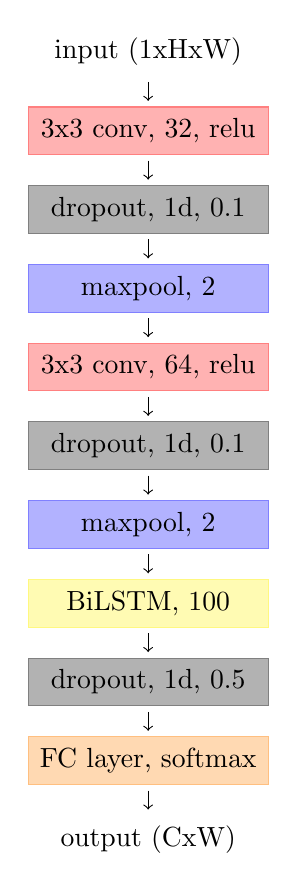
\begin{tikzpicture}[node distance = 1cm]
        \tikzset{
          base/.style={draw, align=center, minimum height=4ex, rectangle, text centered},
          proc/.style={base, draw=white, rectangle, text width=8em},
          conv/.style={proc, draw=red!50, fill=red!30},
          maxp/.style={proc, draw=blue!50, fill=blue!30},
          drop/.style={proc, draw=black!50, fill=black!30},
          lstm/.style={proc, draw=yellow!50, fill=yellow!30},
          soft/.style={proc, draw=orange!50, fill=orange!30},
          line/.style={draw, shorten <= 2pt, shorten >= 2pt, ->}
        }
        \node [proc] (input) {input (1xHxW)};
        \node [proc, conv, below of=input] (conv1) {3x3 conv, 32, relu};
        \node [proc, drop, below of=conv1] (drop1) {dropout, 1d, 0.1};
        \node [proc, maxp, below of=drop1] (maxp1) {maxpool, 2};
        \node [proc, conv, below of=maxp1] (conv2) {3x3 conv, 64, relu};
        \node [proc, drop, below of=conv2] (drop2) {dropout, 1d, 0.1};
        \node [proc, maxp, below of=drop2] (maxp2) {maxpool, 2};
        \node [proc, lstm, below of=maxp2] (lstm1) {BiLSTM, 100};
        \node [proc, drop, below of=lstm1] (drop3) {dropout, 1d, 0.5};
        \node [proc, soft, below of=drop3] (softm) {FC layer, softmax};
        \node [proc, below of=softm] (output) {output (CxW)};

        \path [line] (input) -- (conv1);
        \path [line] (conv1) -- (drop1);
        \path [line] (drop1) -- (maxp1);
        \path [line] (maxp1) -- (conv2);
        \path [line] (conv2) -- (drop2);
        \path [line] (drop2) -- (maxp2);
        \path [line] (maxp2) -- (lstm1);
        \path [line] (lstm1) -- (drop3);
        \path [line] (drop3) -- (softm);
        \path [line] (softm) -- (output);

        \end{tikzpicture}
        \captionof{figure}{Network architecture ($H$: sequence height, $W$: sequence length, $C$: alphabet size)}
        \label{fig:kraken_arch}
\end{wrapfigure}

\section{Kraken}

The Kraken text recognition engine is an extensively rewritten fork of the
OCRopus system. It can be used both for handwriting and printed text
recognition, is easily (re-)trainable, and great care has been taken to
eliminate implicit assumptions on content and layout that complicate the
processing of non-Latin and non-modern works.

Thus Kraken has been extended with features and interfaces enabling the
processing of most scripts, among them full Unicode right-to-left,
bidirectional, and vertical writing support, script detection, and multiscript
recognition. Processing of scripts not included in Unicode is also possible
through a simple JSON interface to the codec mapping numerical model outputs to
characters. The same interface provides facilities for efficient recognition of
large logographic scripts.

Output includes fine-grained bounding boxes down to the character level that
may be used to quickly acquire a large number of samples from a corpus to
assist in paleographic research. Kraken implements a flexible output
serialization scheme utilizing a simple templating language. Templates are
available for the most commonly used formats ALTO, hOCR, TEI, and abbyyXML.


While including implementations of all the subprocesses needed in a text
recognition pipeline, most functional blocks can be accessed separately on the
command line, allowing flexible substitution of specially optimized methods.  A
stable programming interface allows total customization and integration into
other software packages.

\subsection{Recognition}

The recognition engine operates as a segmentation-less sequence classifier
using an artificial neural network to map an image of a single line of text,
the input sequence, into a sequence of characters, the output sequence. The
artificial neural network employed is a combination convolutional and recurrent
neural network trained with the CTC loss function
\cite{graves2006connectionist} that reduces training data requirements to
line-level transcriptions (figure~\ref{fig:kraken_transcription}). Regularization is
mainly provided by dropout \cite{hinton2012improving} after both convolutional
and recurrent layers. User intervention in determining training duration and
model selection is largely eliminated through early stopping.

\begin{wrapfigure}{O}{0.5\textwidth}
	\includegraphics[width=0.8\linewidth]{88bf936743d1a444d5c0d85be2449a0d.jpg}
	\centering
	\captionof{figure}{Sample output of the trainable segmentation method}
	\label{fig:kraken_seg}
\end{wrapfigure}

Specialized networks, e.g. for particularly complex scripts, can be assembled
from building blocks with a simple network specification language although the
default architecture shown in figure~\ref{fig:kraken_arch} is suitable for the vast
majority of applications.

Processing of dictionaries and library catalogues with extensive semantic
markup such as italic, underlining, and bolding, is also possible through
specially prepared training data.

\subsection{Layout Analysis and Script Detection}

Kraken's layout analysis extracts text lines from an input image for later
processing by the recognition engine. Apart from a basic segmenter taken from
OCRopus a trainable line extractor is in the process of being implemented. Full
trainability of layout analysis is of utmost importance to a truly universal
OCR system, as text layout and its semantics varies widely across time and
space, e.g. hand-crafted methods for printed Latin text are unlikely to work
reliably on Arabic text or manuscripts with extensive interlinear annotation.

The trainable layout analysis module consists of a two-step instance
segmentation method: an initial seed-labelling network operates on the whole
page labelling the area between baseline and mean of each line. As the output
of the network is a probability of each pixel belonging to a baseline it is
binarized using hysteresis thresholding after smoothing with a gaussian filter.
The binarized image is then skeletonized and end point are extracted with a
discrete convolution. Finally, the vectorized baseline between the endpoints is
rectified and a variable environment calculated based on the distance of
connected components from the labelled area is extracted.

\begin{table}[h]
\centering
\begin{minipage}{\textwidth}
\caption{Mean character accuracy and standard deviation on the validation set
	across 10 training runs on each training set}
\label{tab:kraken_acc}
\renewcommand\footnoterule{}
\begin{tabularx}{\textwidth}{lXXX} \toprule
& \textbf{Mean character accuracy} & \textbf{Standard deviation} & \textbf{Maximum accuracy}\\
\addlinespace
\textbf{Prints}\ \\ \midrule
Arabic~\cite{kiessling2017important} & 99.5\% & 0.05 & 99.6\%\\
Persian\footnote{Mid-20th century printing} & 98.3\% & 0.33 & 98.7\%\\
Syriac\footnote{Late-19th century printing in Serṭā form}& 98.7\% & 0.38 & 99.2\%\\
Polytonic Greek\footnote{Late-19th century printing}& 99.2\% & 0.26 & 99.6\%\\
Latin~\cite{springmann2018ground} & 98.8\% & 0.09 & 99.3\%\\
Latin incunabula~\cite{springmann2018ground} & 99.0\% & 0.11 & 99.2\%\\
Fraktur~\cite{springmann2018ground} & 99.0\% & 0.31 & 99.3\%\\
Cyrillic\footnote{1923 Russian print}& 99.3\% & 0.15 & 99.6\%\\
\addlinespace
\textbf{Manuscripts}\ \\ \midrule
Hebrew\footnote{Medieval Midrash Tanhuma}& 96.9\% & - & -\\
Medieval Latin\footnote{Mid-9th century Carolingian of Josephus Latinus} & 98.2\% & -  & -\\
\bottomrule
\end{tabularx}
\end{minipage}
\end{table}

The seed-labelling network is a modified U-net \cite{ronneberger2015u} on the
basis of a 34-layer residual network \cite{he2016deep} pretrained on ImageNet.

Preliminary results on a page from a publicly available dataset of Arabic and
Persian manuscripts \cite{kiessling2019badam} can be seen in
Figure~\ref{fig:kraken_seg}.

\begin{figure}[h!tp]
	\includegraphics[width=0.8\linewidth]{high.png}
	\centering
	\captionof{figure}{Sample output of the script detection on a bilingual
	French/Arabic page. Note that Eastern Arabic are always classified as
	Latin text}
	\label{fig:kraken_script}
\end{figure}

Script detection, the basis for multi-script support in the recognizer, is
implemented as a segmentation-less sequence classification problem, similar to
text recognition. Instead of assigning a unique label to each code point or
grapheme cluster we assign all code points of a particular script the same
label. The network is then trained to output the correct sequence of script
labels (figure~\ref{fig:kraken_transcription}). The output sequence is then
used to split the line into single-script runs that can be classified with
monolingual recognition models (figure~\ref{fig:kraken_script}).

\begin{figure}[h]
        \includegraphics[width=\linewidth]{transcription.png}
        \centering
        \captionof{figure}{Original and modified ground truth (top: original line, middle: transcription,\\ bottom: assigned script classes)}
        \label{fig:kraken_transcription}
\end{figure}

\section{Results}

Kraken has been used on a wide variety of writing systems, achieving uniformly
high character accuracy (CER). Sample accuracies for a diverse set of scripts
spanning across multiple centuries of printing are shown in table
\ref{tab:kraken_acc}. It should be noted that recent improvements in the text
recognition engine result in significantly diminished character error rates in
comparison to earlier versions such as those evaluated in
\cite{kiessling2017important}.

As a special use case we evaluated recognition of text and emphasis in a mixed
English and romanized Arabic library catalog on a training set of 350 lines (50
lines in the validation set) resulting in an averaged CER  of 99.3\%
($\sigma=0.16$) over 10 runs with 95.38\% CER on cursive and text with
increased spacing ($\sigma=1.46$). When using only emphasized text accuracy as
the stopping criterium mean accuracy rises to 99.03\%
($\sigma=0.28$)~\cite{kiessling2018read}.
